% !TEX TS-program = pdflatex
% !TEX encoding = UTF-8 Unicode

% This is a simple template for a LaTeX document using the "article" class.
% See "book", "report", "letter" for other types of document.

\documentclass[11pt]{article} % use larger type; default would be 10pt

\usepackage[utf8]{inputenc} % set input encoding (not needed with XeLaTeX)
\usepackage{listings}
\usepackage{color}
\usepackage[utf8]{inputenc}

% Default fixed font does not support bold face
\DeclareFixedFont{\ttb}{T1}{txtt}{bx}{n}{12} % for bold
\DeclareFixedFont{\ttm}{T1}{txtt}{m}{n}{12}  % for normal

% Custom colors
\usepackage{color}
\definecolor{deepblue}{rgb}{0,0,0.5}
\definecolor{deepred}{rgb}{0.6,0,0}
\definecolor{deepgreen}{rgb}{0,0.5,0}

\usepackage{listings}

% Python style for highlighting
\newcommand\pythonstyle{\lstset{
language=Python,
basicstyle=\ttm,
otherkeywords={self},             % Add keywords here
keywordstyle=\ttb\color{deepblue},
emph={MyClass,__init__},          % Custom highlighting
emphstyle=\ttb\color{deepred},    % Custom highlighting style
stringstyle=\color{deepgreen},
frame=tb,                         % Any extra options here
showstringspaces=false            % 
}}


% Python environment
\lstnewenvironment{python}[1][]
{
\pythonstyle
\lstset{#1}
}
{}

% Python for external files
\newcommand\pythonexternal[2][]{{
\pythonstyle
\lstinputlisting[#1]{#2}}}

% Python for inline
\newcommand\pythoninline[1]{{\pythonstyle\lstinline!#1!}}


%%% Examples of Article customizations
% These packages are optional, depending whether you want the features they provide.
% See the LaTeX Companion or other references for full information.

%%% PAGE DIMENSIONS
\usepackage{geometry} % to change the page dimensions
\geometry{letterpaper} % or letterpaper (US) or a5paper or....
% \geometry{margin=2in} % for example, change the margins to 2 inches all round
% \geometry{landscape} % set up the page for landscape
%   read geometry.pdf for detailed page layout information

\usepackage{graphicx} % support the \includegraphics command and options
\usepackage{hyperref}
% \usepackage[parfill]{parskip} % Activate to begin paragraphs with an empty line rather than an indent

%%% PACKAGES
\usepackage{booktabs} % for much better looking tables
\usepackage{array} % for better arrays (eg matrices) in maths
\usepackage{paralist} % very flexible & customisable lists (eg. enumerate/itemize, etc.)
\usepackage{verbatim} % adds environment for commenting out blocks of text & for better verbatim
\usepackage{subfig} % make it possible to include more than one captioned figure/table in a single float
% These packages are all incorporated in the memoir class to one degree or another...

%%% HEADERS & FOOTERS
\usepackage{fancyhdr} % This should be set AFTER setting up the page geometry
\pagestyle{fancy} % options: empty , plain , fancy
\renewcommand{\headrulewidth}{0pt} % customise the layout...
\lhead{}\chead{Serena Booth $\bullet$ Privacy \& Technology}\rhead{}
\lfoot{}\cfoot{\thepage}\rfoot{}

%%% SECTION TITLE APPEARANCE
\usepackage{sectsty}
\allsectionsfont{\sffamily\mdseries\upshape} % (See the fntguide.pdf for font help)
% (This matches ConTeXt defaults)

%%% ToC (table of contents) APPEARANCE
\usepackage[nottoc,notlof,notlot]{tocbibind} % Put the bibliography in the ToC
\usepackage[titles,subfigure]{tocloft} % Alter the style of the Table of Contents
\renewcommand{\cftsecfont}{\rmfamily\mdseries\upshape}
\renewcommand{\cftsecpagefont}{\rmfamily\mdseries\upshape} % No bold!
\usepackage{setspace}

%%% END Article customizations

%%% The "real" document content comes below...

\title{Got Juice? \\ Juice-jacking Maxwell Dworkin Attendees}
\author{CS105: Privacy and Technology \\ Serena Booth}
\date{December 11, 2015} % Activate to display a given date or no date (if empty),
         % otherwise the current date is printed 


\begin{document}
\maketitle
\doublespacing
{
\centering
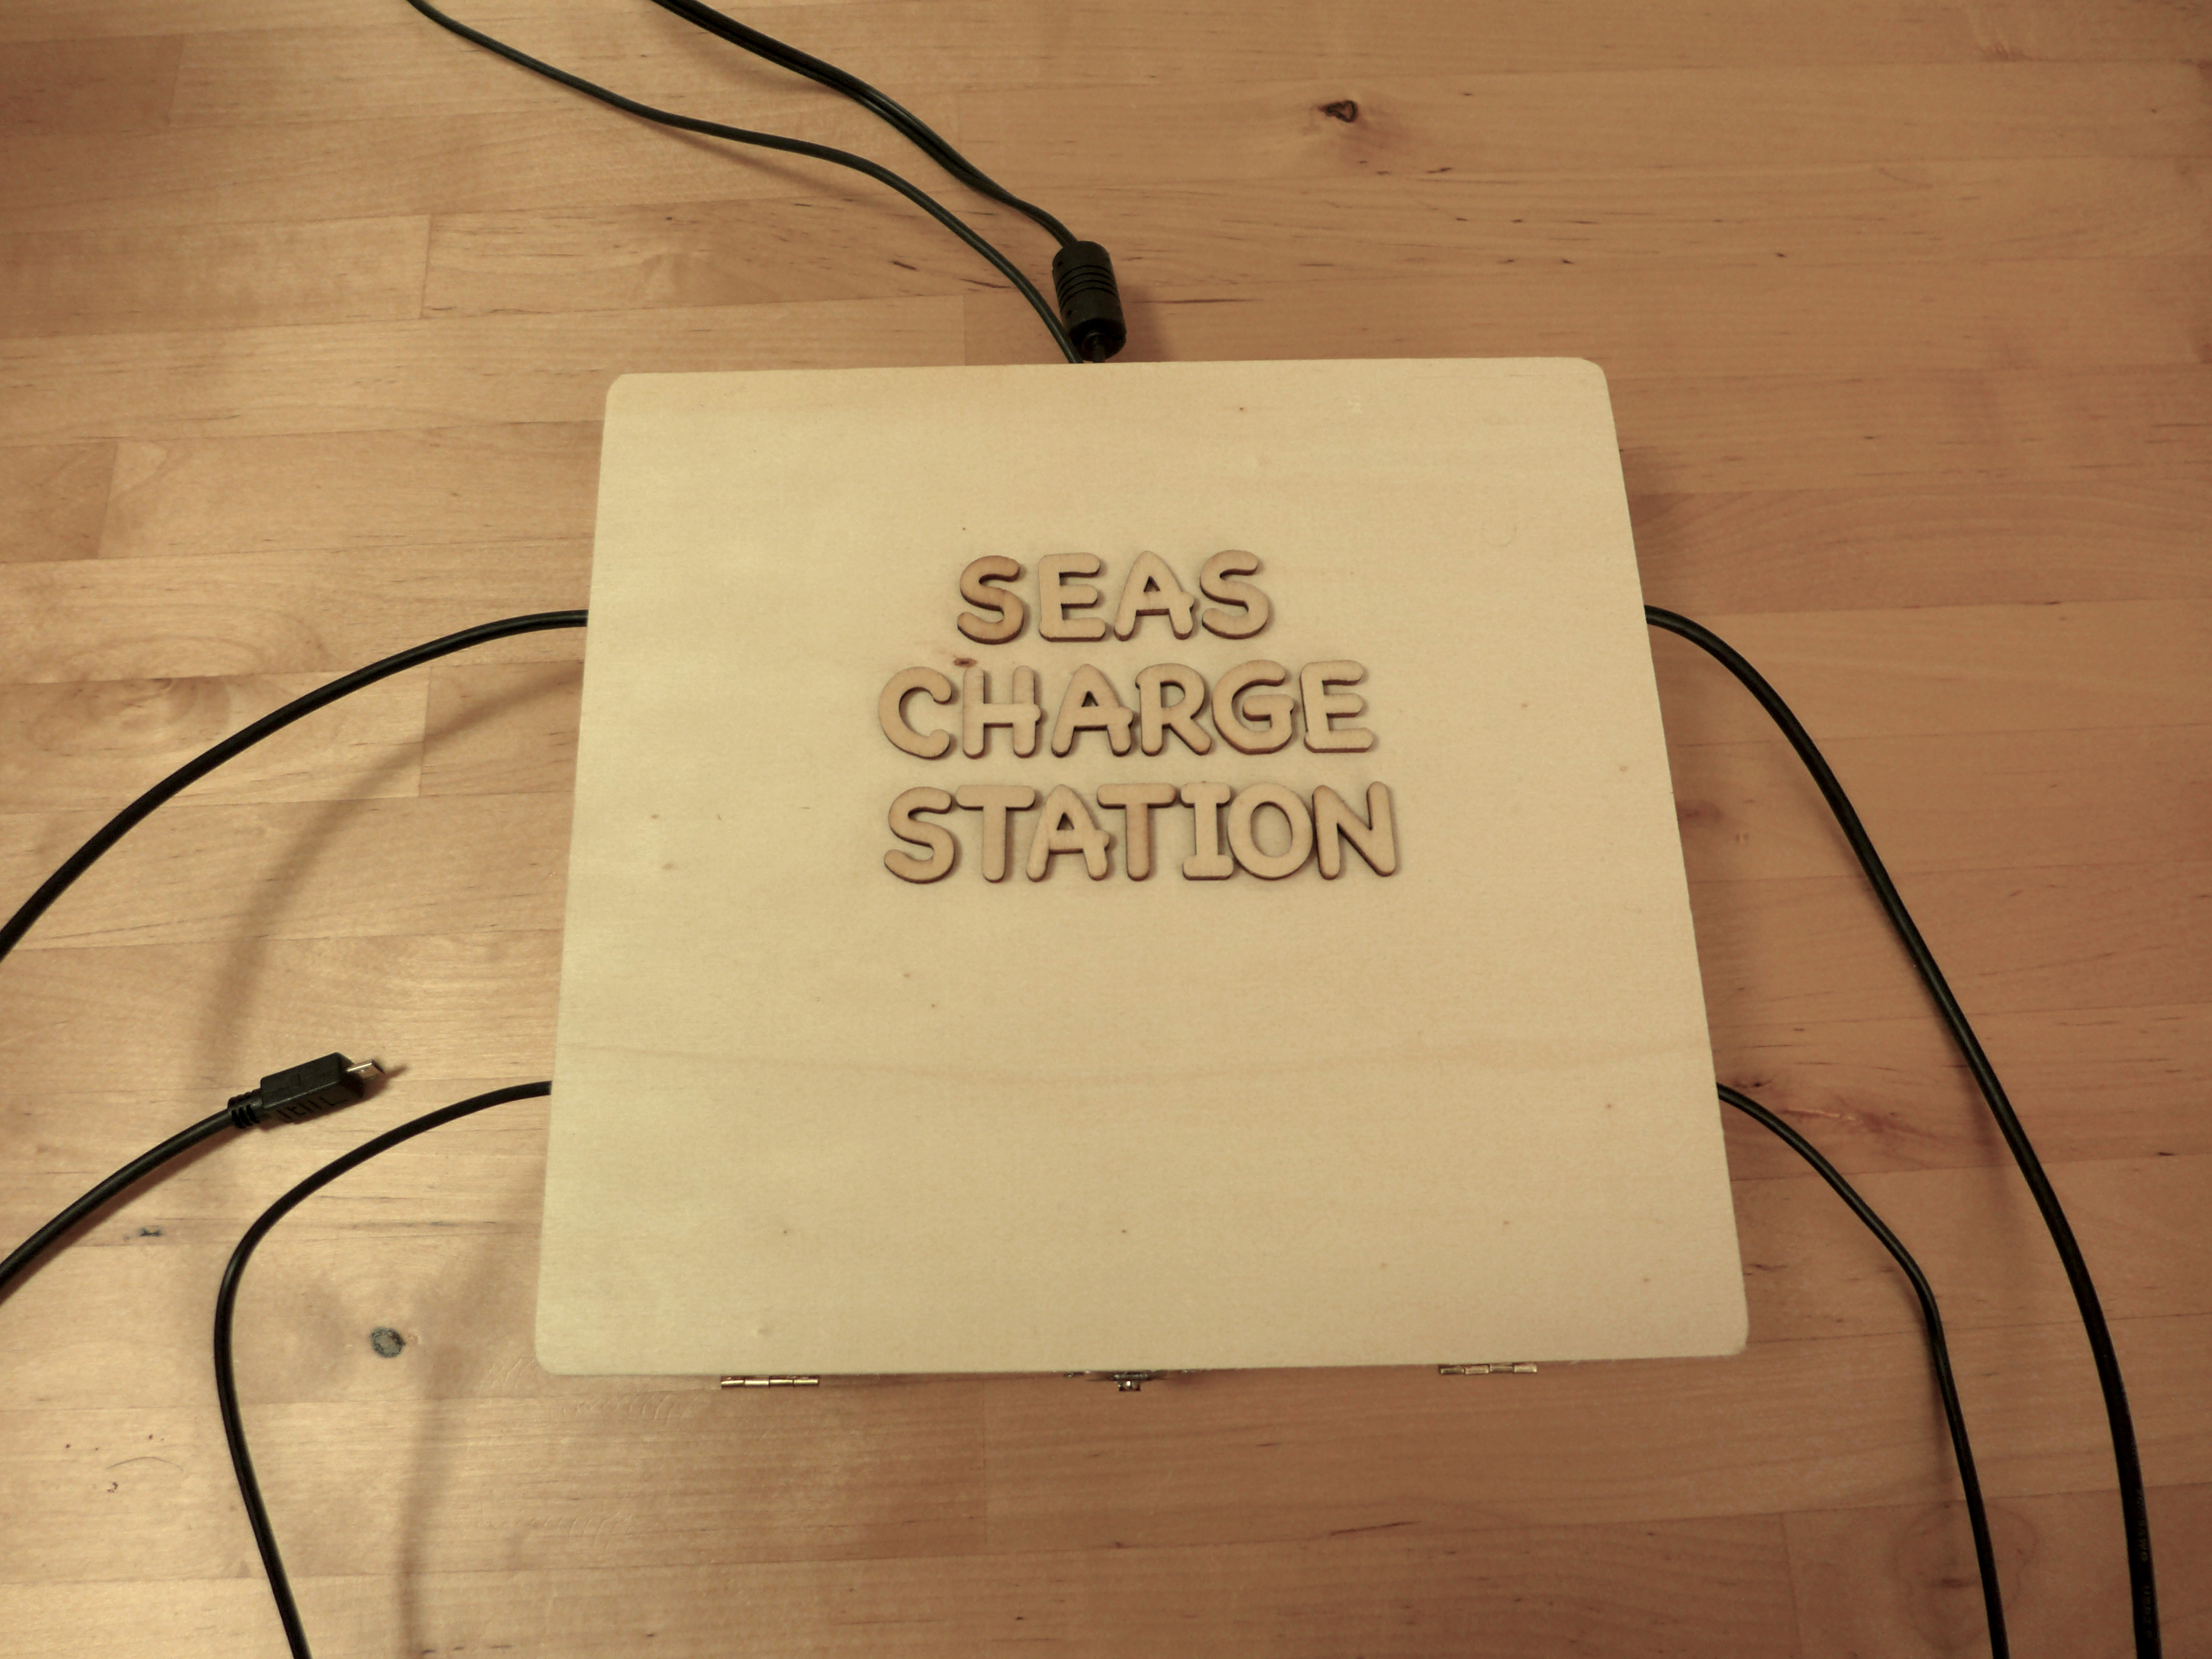
\includegraphics[width=\textwidth]{photo}
}
\section{Abstract}

Batteries are unable to keep up with smartphone usage. In response to the low battery epidemic, many social centers and shopping destinations have set up ``charge stations,'' consisting of powered common phone charging cables. These charging stations represent a privacy threat, as most phone charging cables facilitate both a data and power connection. 

\section{Introduction}

Because phone charging cables transmit data, smartphone OS designers and distributors have created defenses against so-called ``juice-jacking,'' wherein an assailant without authorization either retrieves data or injects malware when a user charges their phone. However, as is often the case in the world of privacy and technology, these protections against juice-jacking detract from convenience. I thus created a rogue charging station which encourages users to embrace convenience over data protection. I deployed this charging station in the second floor student lounge of Maxwell Dworkin, the Harvard computer science building. 

\section{OS Protections} 

Each smartphone operating system has a suite of protections in place against juice-jacking. Here, I analyze the main lines of defense and limitations for three such operating systems. 

\subsection{iOS} 

\begin{itemize}
\item As of iOS 7, Apple employs two major protections against juice-jacking. First, an iOS device's data connection is entirely powered down when the phone is locked. Second, on an attempted data connection, an iOS device presents a prompt asking the user to `Trust this Computer?' If the user responds, `Don't Trust,' the data connection remains disabled; if instead the user responds, `Trust,' the data connection is enabled. 

\item The iOS notification asking users to `Trust this Computer?' is flawed and can be  manipulated. First, the word choice is questionable: people generally regard themselves to be trusting, so this notification toys with human psyche. Second, the meaning of ``trust'' is entirely opaque to a layman, as data connection and communication is opaque. Third, and most importantly, this notification is annoying. Dozens of websites are devoted to instructing iOS users to prevent the notification from appearing. 
\end{itemize} 

\subsection{Android} 

\begin{itemize}
\item Android Ice Cream Sandwich and later likewise employ two major protections. Most Android handsets have their data connection disabled when the phone is locked. Android has ``MTP,'' or media transfer protocol enabled by default; however, a passive notification is presented to an Android user when this connection is made. MTP and ``PTP,'' an alternate transfer protocol designed for pictures, can be disabled manually. 

\item Androids' default settings make these phones vulnerable to juice-jacking. While the user is alerted when a data connection between a computer and the phone is active, the user's data has already been compromised, even if the user then disables MTP. 
\end{itemize} 

\subsection{Windows} 

\begin{itemize}
\item Windows handsets protect against juice-jacking by limiting a response to a data request when the device is locked. This strategy is unique among the OS competition. 

\item In providing a partial response to a data request, Windows exposes the layout of the phone's data, even when the phone is locked. This information can be used to access a remote storage device (such as a microSD card) if used with the handset\footnote{Windows Phone 8.1 must be configured to enable data-at-rest protection for removable storage media or to disable the removable storage media. \url{https://www.stigviewer.com/stig/microsoft_windows_phone_8.1/2015-05-13/finding/V-58947}}. Further, as of Windows 8, users were not able to encrypt the contents of this additional storage. 
\end{itemize} 

\section{Materials and Methods}

At the 2011 Defcon conference, one ``hacker'' presented a rogue charging station. Over the course of the week-long conference, 360 attendees used this charging station\footnote{Beware of Juice-Jacking, \url{http://krebsonsecurity.com/2011/08/beware-of-juice-jacking/}}. In 2013, researchers at Geogia Tech presented a rogue charger which was capable of injecting malware onto an iOS device in under a minute\footnote{Mactans: Injecting Malware into iOS devices via Malicious Chargers, \url{https://media.blackhat.com/us-13/US-13-Lau-Mactans-Injecting-Malware-into-iOS-Devices-via-Malicious-Chargers-WP.pdf}}. Thus juice-jacking has been exposed as a risk since 2011, and the above obstacles to juice-jacking have been implemented since then. In designing my rogue charging station, I wanted to see which protections users would compromise -- particularly, if users would unlock their phones -- for the sake of  convenience.  

\subsection{Materials} 

I purchased the following materials in order to assemble the rogue charging station: 
\begin{itemize}
\item 2x USB micro charging cables (Android + Windows devices) 
\item 2x USB lightning charging cables (iOS devices) 
\item A self-powered USB hub
\item A USB splitter
\item A Raspberry Pi
\item A 32GB SD card
\end{itemize} 

\subsection{Methods} 

I wrote a program which sends me an email if a USB device was connected with an enabled data connection. In particular, in the case of an Android or iOS device, this meant that a user was not only charging their device from my rogue unit, but had given up their first line of defense against juice-jacking: they had unlocked their phone. In order to facilitate such interactions, I placed the charging device on a study table, hoping that users would sit at the table and thumb through their phone while connected. Likewise, I selected 3' USB cables to enable this interaction mode. If my charging station is unplugged, it will restart the usb counting script on startup. If an error occurs when running the script, the script simply ignores the error. If the script is killed, it is relaunched by a helper application.\\

\noindent Being a miscreant, I also wanted to determine whether users of my charging station had yielded all data protections. I focused on Android users in this endeavor, as iOS uses a proprietary transfer protocol. When an Android device is connected to my charging station, I attempt to enable an MTP connection. If that connection is successful, I search the user's phone for a folder entitled ``DCIM.'' If such a folder is found and is accessible to me, I disconnect from MTP and email myself a notification that a user has effectively given me access to all of the photographs on their phone. While I considered posting three random pictures to Twitter in response to such an event, I realized this would overstep.

\section{Results}

As of December 11, 21 users have used my charging station and yielded their first line of defense by unlocking their phones. The charging station has been in operation since November 30. Of the 21 devices, 19 were iPhones; 1 an LG, 1 a Samsung Galaxy. The LG device had MTP disabled, but the Samsung device allowed me to access its DCIM folder. 

\section{Defense Against The Dark Arts}

Simple steps can protect users from juice-jacking. I enumerate those steps here: 

\begin{enumerate}
\item Avoid using charging stations! 
\item When using a charging station, power your phone down. 
\item When using a charging station, do not unlock your phone. 
\item iOS users should not trust computers, except their personal machine for syncing data. 
\item Android users should disable MTP and PTP unless syncing data. 
\item All users should wear a ``USB condom''\footnote{Available for \$4.99 from SyncStop, \url{http://shop.syncstop.com/collections/buy/products/usb-condom?variant=808433739}} when charging their devices. 

\end{enumerate}

\section{Conclusion}

Juice-jacking has potential to compromise data security on smartphones. Photographs can be stolen, malware can be injected. In a lounge devoted to computer science students, 21 attendees have compromised the protections that their smartphone OS'es offer for the sake of powering up. Maxwell Dworkin has relatively small throughput, and most attendees bring computers and their own USB cables with them. Given that in this small, controlled environment, I saw significant charge use, I posit that a rogue charging station could wreak havoc in a heavily attended location such as an airport or a popular shopping destination. 

\newpage
\appendix
\section{Appendix: Deployed Code}\label{App:AppendixA}

Thanks to \url{http://stackoverflow.com/questions/8110310/} and \url{https://drautb.github.io/2015/07/27/the-perfect-exchange-mtp-with-python/}
\pythonexternal{usbcounter.py}

\newpage
\section{Appendix: Q\&A from Class Presentation}\label{App:AppendixB}

\begin{itemize} 
\item Q: Is there a difference between plugging in your own specific USB chord and using a charging station that has one already? (Does a charging station with its own USB give it a higher probability of acquiring more data?)

A: There are two types of USB cables: one type transmits both power and data, another transmits only power. If you carry a power-only cable, you are indeed protected in much the same way as you would be if you used a USB condom. However, if you carry a data cable (and most USB cables are data cables), you are not afforded any protections. 

\item Q: If android debugging is enabled, I would very much like to see some test installation of root-access applications that can then hide on the device. If it can be done quickly, that would be amazing! (Also phone will not have to be unlocked) I am also curious what proportion of user's phones are unlocked. 

A: Indeed, this would be a very interesting follow up to my work. Sadly, for a charging station deployed in Maxwell Dworkin, I believe this experiment would not turn up many results. Of the 20 phones used with the charging station to date, 19 have been iPhones. That said, previous research has demonstrated that with an iPhone which has given ``trust'' to a computer, malware can be injected in less than a minute\footnote{Mactans: Injecting Malware into iOS devices via Malicious Chargers, \url{https://media.blackhat.com/us-13/US-13-Lau-Mactans-Injecting-Malware-into-iOS-Devices-via-Malicious-Chargers-WP.pdf}}. 

\item Q: What is the maximum threat once you gain access? How much data could you collect, and would that impact people beyond just the phone accessed? (for example phone numbers and contact names of other individuals)

A: The threat is significant. If you're able to gain access to the phone in this capacity, the phone's data is presented to you in an unencrypted form. You can immediately take any information from the phone which is designed to by synced between phones and computers -- all media and contacts. Moreover, this attack enables the injection of malware onto the phone, as the data communication is two-way. Such an attack was demonstrated by Geogia Tech in 2013\footnote{Ibid.}. 

\item What is and isn't illegal surrounding what information can be used/taken from your phone when it is unlocked in a changing station? Are the privacy attacks something that can be done or is legal to do?

A: I haven't thoroughly investigated the legal issues around this technology. I would hazard a guess that so long as a terms of use is viewable, a malicious charger which retrieves data from the device is permissible, while a malicious charger which injects malware is not. 

\item Q: Your project was fascinating and I will certainly never use charging kiosks again. But in my mind, your project raises a lot of questions, specifically regarding regulation of operating a charging kiosk. Since many people (including myself before today) had no clue that connecting to a kiosk and operating my phone could put my data at risk, should the government step in and "protect" people by banning these charging kiosks (unless they explicitly inform the people using it through a sign.) Its essentially the opt-in/opt-out debate regarding informed consent.

A: Public charging kiosks provide an extremely useful service, so I am not in the least bit opposed to them. My suggested reform is with smartphone operating systems. I believe Apple is on the right track with their ``Trust this Computer?'' notification before enabling a data connection. With better wording, and perhaps a less annoying notification which defaulted to a non-trusting state, this protection could ensure that rogue charging stations posed a very limited threat. 

\item Q: Very interesting work—I agree that most people simply ignore the risk associated in connecting their phone to charge at a charging station. Do you know if there are any statistics that show that this goes beyond the theoretical field and that some of these charging stations do, in fact, contain computers in them that are capable of gathering information? It'd be interesting to see whether it is a documented attack. Also, to your knowledge, how often do you think charging kiosks collect data from phones? It is clear from your presentation that this data collection is possible, but is it implemented?

A: Researchers speculate that this type of attack has not been launched in any substantial form to date. In 2011, a Defcon participant presented a malicious charger at the hacking conference, and saw 360 self-labeled ``hackers'' use the charging station over the course of a week\footnote{Beware of Juice-Jacking, \url{http://krebsonsecurity.com/2011/08/beware-of-juice-jacking/}}. 

\item Q: Why were you not able to get at the DCIM folder of these 10 users? Is there another protection in Android that prevents you from doing so? Or were all these 10 users protecting themselves in some way?

A: My MTP attack is only launched on Android users. Of the 10 users prior to the presentation, 9 were iPhone users, and the 1 Android user had MTP disabled. As of December 11th, 20 users have unlocked their phones while engaged with my charging unit. Of those, 19 have been iPhones. 

\end{itemize} 






\end{document}
